\documentclass[../main.tex]{subfiles}

\begin{document}
	
The overview of the proposed solution is depicted in 
\cref{fig:solution-overview}. 
The following subsections will
explain in more detail why this solution is chosen
and what the integral components are.

\begin{figure}[tbp]
	\centering
	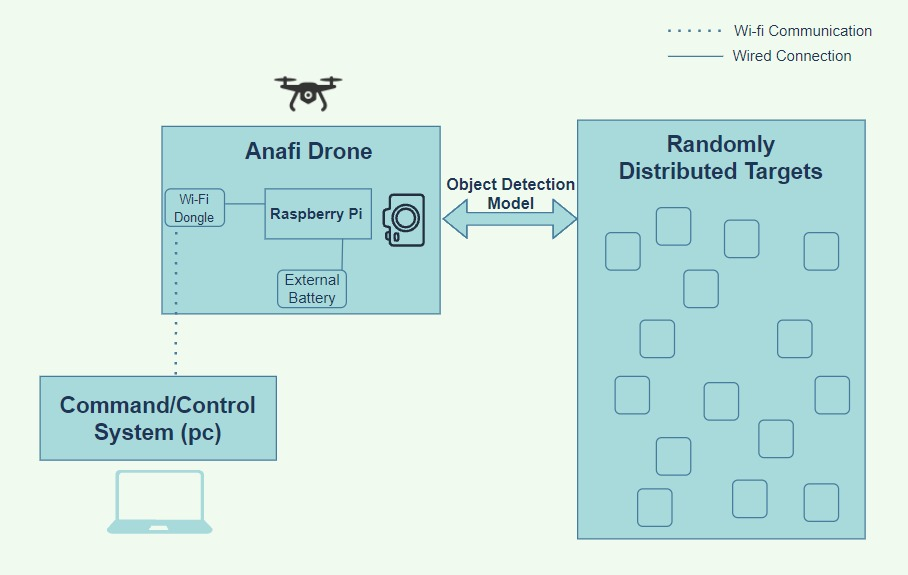
\includegraphics[width=0.9\textwidth]{diagram.jpeg}
	\caption{A general overview of the solution.}
	\label{fig:solution-overview}
\end{figure}

\subsection{Alternative solutions and tradeoffs}

\begin{table}[H]
    \centering
    \caption{A comparison of the alternative solutions.}
    \label{tab:alt-solutions}
    \begin{tabular}{ p{4cm} p{6cm} p{6cm} }
        \toprule
        \textit{} & \textit{Design A} & \textit{Design B}\\ \midrule
        Type  & Custom made drone with onboard computer & Commercial drone with high performance and many features    \\
        Flexibility & Very flexible and customization is easy & Hard to customize or modify it since it flies under limited protocols and standards. \\

        Price and Availability & Cheaper but the shipping and building processes must be considered & Expensive but in our case its available in our hands and ready to fly.   \\

        Onboard computer & Must have & Must have \\
        \bottomrule
    \end{tabular}
\end{table} 

From the \cref{tab:alt-solutions} above, 
we can see some tradeoffs 
between design A and design B, but in both designs, 
an onboard microcomputer must be present for 
flying control and the support of autopilot feature. 
There are three options for onboard microcomputers, 
which are shown in the following 
\cref{tab:onboard-computers}. Raspberry Pi 4 seems 
to be the winner since it has advantages 
in specifications, connection interfaces, 
and availability.

\begin{table}[bt]
    \centering
    \caption{A comparison of the onboard computers.}
    \label{tab:onboard-computers}  
    \begin{tabular}{ p{3cm} p{4cm} p{4cm} p{4cm} }
        \toprule
        \textit{} & \textit{Raspberry Pi 4} & \textit{NVIDIA Jetson Nano} & \textit{\textsc{dji} Manifold}\\ \midrule
        Specifications  & CPU:Cortex-A72 (ARM v8) 64-bit@ 1.5GHz | Ram :4GB or 8GB LPDDR4-3200 SDRAM | GPU : Broadcom VideoCore VI & CPU:Quad-core ARM A57 @ 1.43 GHz | Ram: 4 GB 64-bit LPDDR4   | GPU:128-core Maxwell & CPU:Quad-core,ARM | Ram: 2 GB DDR3L | GPU:Low-power GeForce graphics processor \\ \addlinespace
        Connection interfaces & 2.4 GHz and 5.0 GHz IEEE 802.11ac wireless, Bluetooth 5.0 & Gigabit Ethernet \& M.2 Key E (for WiFi support). &10/100/1000 BASE-T Ethernet \\ \addlinespace

        Price \& Availability & 300 QAR available and can be used on any drone & 400 QAR available but need to be ordered and shipped & Very expensive and restricted to \textsc{dji} drones and \textsc{dji} company stopped selling it \\ \addlinespace
        Picture & \begin{minipage}{.2\textwidth}
            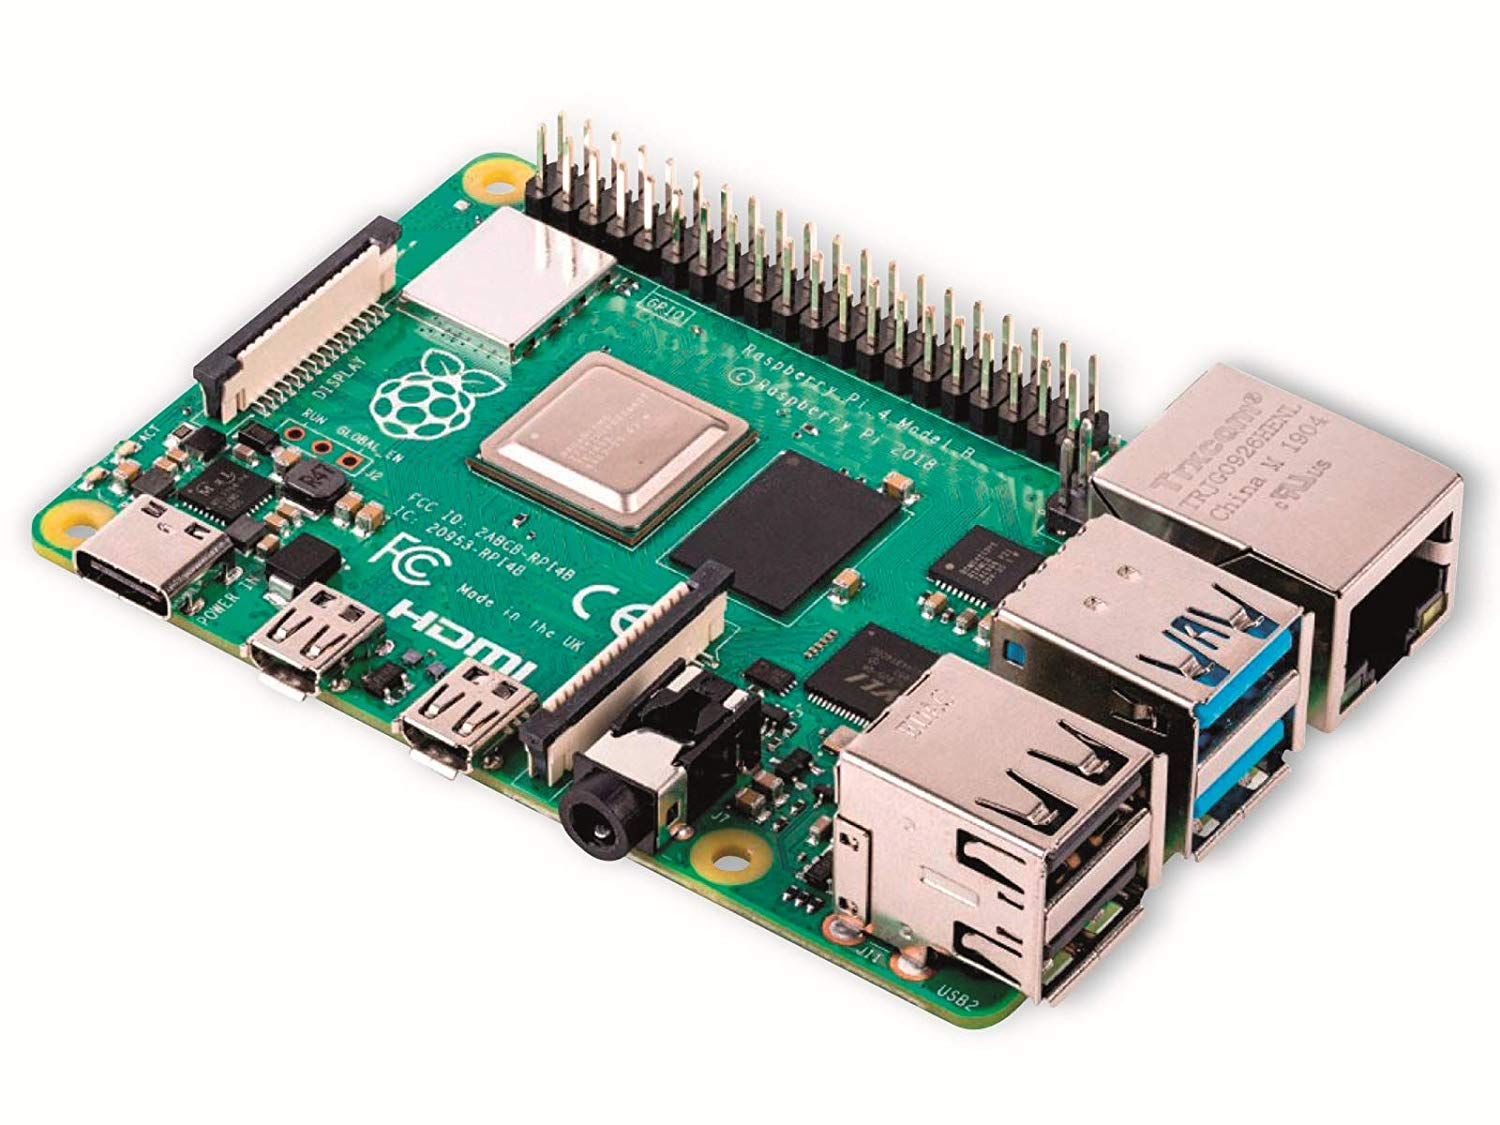
\includegraphics[width=40mm, height=30mm]{raspberry.jpg}
            \end{minipage}  & \begin{minipage}{.2\textwidth}
            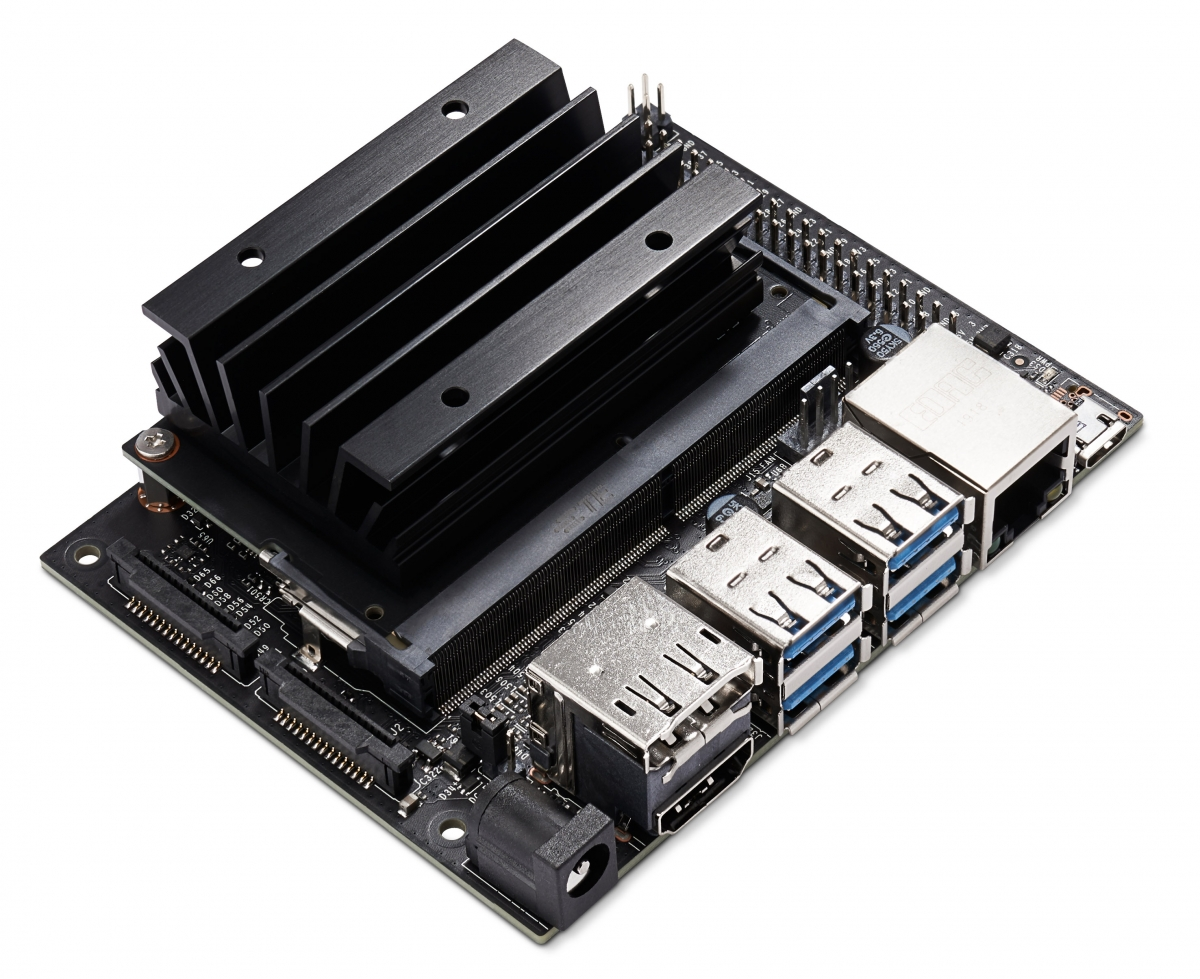
\includegraphics[width=40mm, height=30mm]{jetson.jpg}
            \end{minipage} & \begin{minipage}{.2\textwidth}
            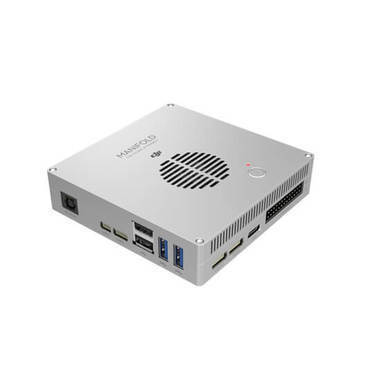
\includegraphics[width=40mm, height=30mm]{manifold.jpg}
        \end{minipage} \\
        \bottomrule
        \end{tabular}
    \end{table}

\subsection{Selected solution overview}\label{sec:selected-solution}

The proposed solution consists of two main parts: 
a commercial drone and a controlling system.
We have chosen the commercial drones especially 
the Parrot \anafi for several reasons.
Firstly, it is supported by a continuously updated 
\textsc{sdk} and it can be controlled easily 
with a simple Python script which makes 
\gls{drl} development much easier and more stable. 

Secondly, it has a good flight time 
as the \anafi drone has a 2700 mAh battery. 
It can fly up to 25 minutes which is good enough 
for our application.
Finally, its support of Wi-Fi 802.11 and \gls{gps} 
features is essential in our project for 
executing scripts and navigation. 

For how the system will work, firstly, the user 
will import or choose the mobility pattern and set
the constraints to the monitor device,
which is a laptop. Then, the laptop will send basic
high-level commands to the drone agent which is a
Raspberry Pi that in turn will apply certain
operations such as start and stop.

Once the user finishes importing the mobility pattern
and starting the drone mission, the drone will
take off and begin visiting areas and scanning for
the most number of mobile targets based on the
trained \gls{drl} model.
The user will keep receiving live updates and the
status of service on the control section using Wi-Fi.
Most of the connections in the system are wireless,
which will have benefits and drawbacks as discussed
in the \cref{sec:hardware-software} below.

\subsection{High level architecture}

\Cref{fig:arch-fig} shows a high-level architecture 
of the complete working system, in which a group 
of connected adapters and devices are combined into 
a single functional system. 
The architecture is composed of three sections namely
interfacing, controlling, and targets. 
The interfacing section contains the drone that 
will handle the onboard computer, its power source, 
and the connection adapters. 
In the controlling part, a personal computer 
will be responsible for contacting the onboard computer 
to adjust settings, execute scripts, and get 
live updates and results. 
Finally, there will be multiple moving targets 
in the target section. For example, 
\textsc{r/c} cars are controlled manually and moving in 
a specific mobility pattern with varying directions 
and destinations. 
In the next section, hardware and software components 
will be presented in a more detailed manner.

\begin{figure}[tbp]
    \centering
    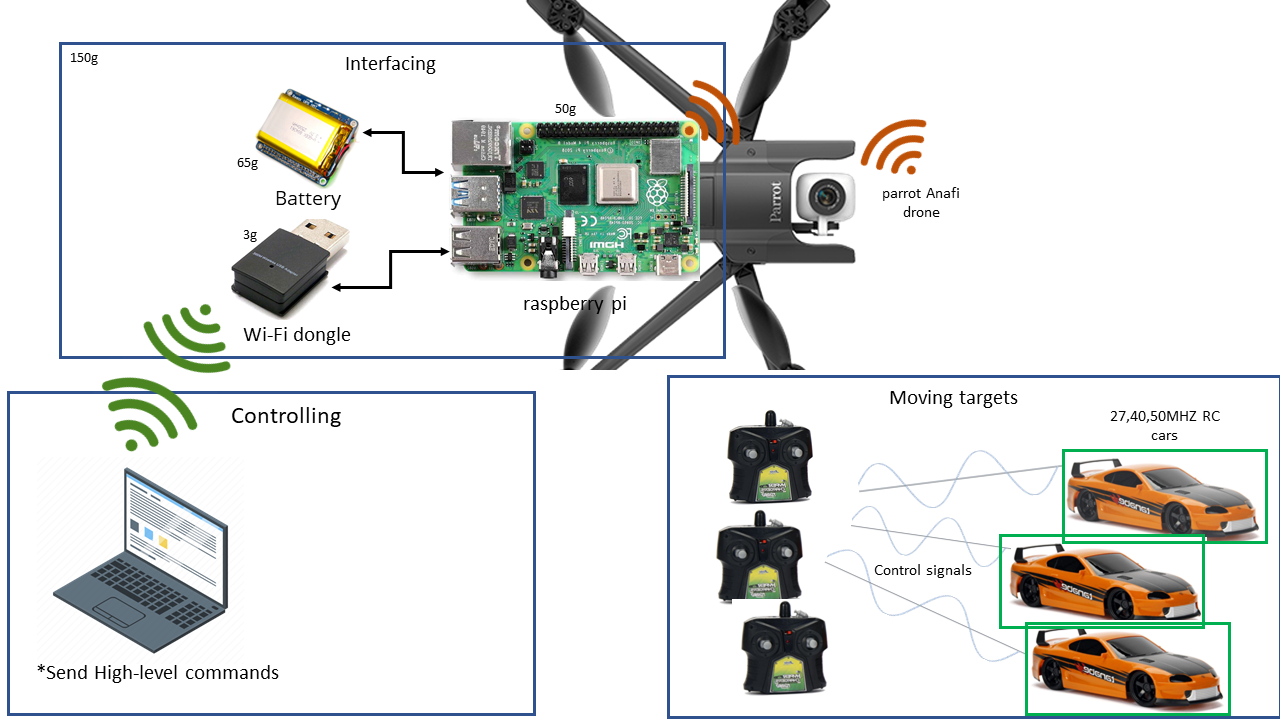
\includegraphics[width=0.9\textwidth]{high-level-arch.png}
    \caption{The high-level architecture of the overall system.}
    \label{fig:arch-fig}
\end{figure}


\subsection{Hardware/software to be used}\label{sec:hardware-software}

\subsubsection{Software}
    %parrot olympe
    %parrot sphinx
    %Gazebo simulator
    %roboflow
    %google colab notebook 
    %jupyter notebook
There are three primary categories of software 
depending on the usage: simulation, training, 
and application and they are listed in \cref{tab:software-used}. The first part will focus on 
simulating the environment, testing the models, 
and flight control. Before discussing the software 
to be used, we have selected Ubuntu 18.04 (Bionic Beaver) 
as an operating system for several reasons. 
One key reason is that in addition to
still being supported, it is compatible with the 
Parrot's Olympe and Sphinx programs, which are only 
supported on limited distributions and operating systems.
Another reason is that it is a lite \textsc{os} 
and can be installed on the onboard computer that 
will be attached to the drone. For the simulation part, 
using Sphinx and Gazebo software is a very helpful
to visualize the environment, control the drone, 
and apply the \gls{drl} model. Sphinx is a simulation 
tool built on top of Gazebo 
to run the Parrot's drone firmware on 
personal computers, which comes with helpful 
features for simulation such as visualizing flight 
data at runtime, running the \gls{uav} remotely, 
and executing scripts with the command line. 
Gazebo is a robot \textsc{gui} simulation 
which simulates the visual and physical surrounding 
of drones and custom 3D objects. 
\Cref{fig:gazebo} shows how the Sphinx 
program looks like. 

\begin{table}[tbp]
    \centering
    \caption{Software used in the project.}
    \label{tab:software-used}  
    \begin{tabular}{ p{3cm} p{3cm} p{6cm} }
        \toprule
        \textit{Software} 
            & \textit{Logo} 
                & \textit{Justification} \\ 

        \midrule

        Parrot Olympe  
            & 
            \raisebox{-0.7\height}
            {
\includegraphics[width=2.7cm]
            {parrot.png}}
                & A controller for the Parrot \anafi 
                drone. It makes controlling 
                the drone possible 
                using a Python script \\
                \addlinespace

        Parrot Sphinx  
            & 
            \raisebox{-0.7\height}
            {
\includegraphics[width=2.7cm]
            {parrot.png}}
                & A simulator for the Parrot \anafi drone.
                It loads the Parrot's drone firmware 
                in the simulation environment.
                It is largely based on Gazebo. \\
                \addlinespace

        Roboflow  
            & 
            \raisebox{-0.9\height}
            {
\includegraphics[width=2.4cm]
            {roboflow.png}}
                & A framework for Computer Vision
                development that can be used online.
                It facilitates labelling of images, 
                splitting and merging datasets, 
                applying image transformations 
                and filters, 
                and generating a link for 
                the augmented datasets 
                which will be used in the 
                training notebooks.  \\
                \addlinespace

        Jupyter Notebook  
            & 
            \raisebox{-0.9\height}
            {
\includegraphics[width=2.5cm]{jupyter.png}}
                & A web application for writing, testing 
                and sharing of code. It is free 
                and does not require internet access like 
                the Google Colab. It is used heavily 
                in this project to experiment with new 
                ideas in the Sphinx simulation. \\ 
                \addlinespace

        Google Colab 
            & 
            \raisebox{-0.9\height}
            {
\includegraphics[width=2.8cm]{colab.png}}
                & A Jupyter notebook environment
                running in the cloud. 
                It makes it easy to write, run, 
                and share the code. Most importantly, 
                it gives an option to use remote 
                processing resources in addition to the 
                local ones. \\ 
                \addlinespace

        \bottomrule
    \end{tabular}
\end{table}

\begin{figure}[tbp]
    \centering
    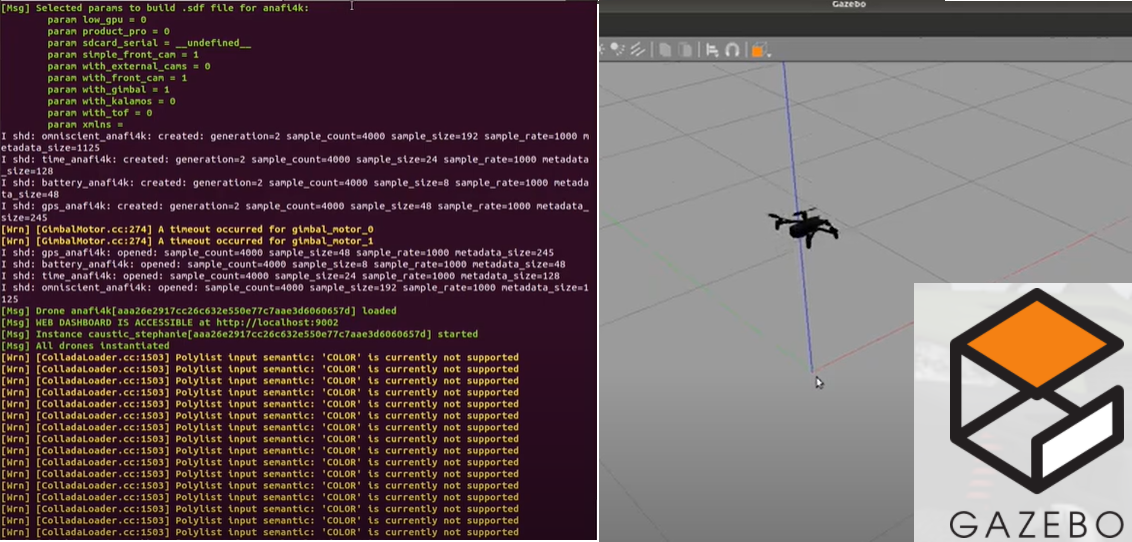
\includegraphics[width=0.9\textwidth]{gazebo.png}
    \caption{The Sphinx program that runs on top of Gazebo.}
    \label{fig:gazebo}
\end{figure}

In the training part, we used simulation tools to 
generate some training datasets. Firstly, 
we placed random objects and captured the images 
using the simulated drone camera. We have used a 
website called Roboflow which helped us labelling 
the objects and generate new datasets from the 
existing ones with different types of augmentation 
such as rotation and scaling. 
For the object detection model, Google Colab notebook 
was a sufficient tool to start training using 
\gls{cnn} \textsc{yolo}v5 in addition to the 
Jupyter notebook which was very helpful 
in code experimentation. 

For the application software, Parrot Olympe 
was used to send commands to the physical as well as 
the simulated drone and control the flight trip and 
how the drone moves. Parrot Olympe uses Python 
controller programming interface for Parrot drones 
which makes controlling simple and easy using a 
Python script. Moreover, Olympe allows us to read
sensor data, such as the \gls{gps} fixes and camera feed, 
from the \anafi
drone. This will make it possible to build a user interface
on the control and command station
shown in \cref{fig:ui-prototype} to monitor 
the progress of the drone
when it is autonomously executing the task visitation
mission.

\begin{figure}[bp]
    \centering
    \includegraphics[width=0.9\textwidth]{ui-prototype}
    \caption{An example of a user interface that will be built
                using sensor data coming from the \anafi drone.}
    \label{fig:ui-prototype}
\end{figure}

\subsubsection{Hardware}
    %Parrot ANAFI Drone
    %Raspberry Pi 4
    %lithium Battery
    %Wi-Fi adapter dongle
    %laptop control station
The main core of the hardware part is the drone, 
which will be the Parrot \anafi. This model 
has a multiple of features that made us choose it 
which have been listed in the 
\cref{sec:selected-solution} above. 
The second important device is the Raspberry Pi 
which will be used as an onboard computer and will 
handle several tasks such as:

\begin{enumerate}
    \item connecting to the drone 
        using a Wi-Fi interface,
    \item controlling the drone 
        by executing Olympe to send control signals 
        to and receive sensory data from the drone,
    \item applying the \gls{drl} model supported by 
        the command and control system,
    \item and receiving high-level commands and 
        sending data to the command and control system.
\end{enumerate}
 
The Parrot \anafi drone is connected 
to the onboard computer using another 
\SI{2.4}{\giga\hertz}
Wi-Fi interface with the help of a 
\SI[per-mode=symbol,per-symbol=p]{300}{MBps} 
Wi-Fi adapter dongle connected to 
the Raspberry Pi through its \textsc{usb} interface. 
Regarding the power source for the Raspberry Pi, 
we thought of taking power directly from the 
drone's battery, but, after some research, we found 
that the \anafi drone's  
socket is somehow different. It is also challenging 
and the drone battery is susceptible to shutting down 
immediately if the voltage reaches less than 3.0 Volt. 
So, we did not want to take the risk and used a 
lithium battery with a power board called 
\textsc{upsp}ack Standard Power Supply attached to 
the main Raspberry Pi board. It includes a 
\SI{4000}{\milli\ampere\hour}
lithium battery, which provides enough power 
and time for our application.

    %Parrot ANAFI Drone
%Raspberry Pi 4
%lithium Battery
%Wi-Fi adapter dongle
%laptop control station
\begin{table}[tbp]
    \centering
    \caption{Hardware used in the project.}
    \label{tab:hardware-used}  
    \begin{tabular}{ p{4cm} p{3cm} p{6cm} }
        \toprule
        \textit{Hardware} 
            & \textit{Picture} 
                & \textit{Justification} \\ 
        
        \midrule

        Parrot \anafi Drone  
            & \begin{minipage}{.1\textwidth}
                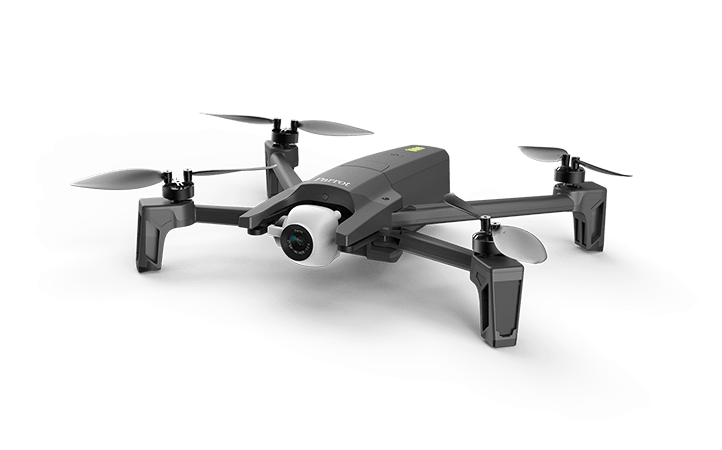
\includegraphics[width=30mm, height=20mm]{anafi.png}
        \end{minipage} 
                & Available in the university, can be 
                controlled easily 
                with simple Python script, 
                4K-high resolution camera.  \\ 
                \addlinespace

        Raspberry Pi 4  
            & \begin{minipage}{.0\textwidth}
                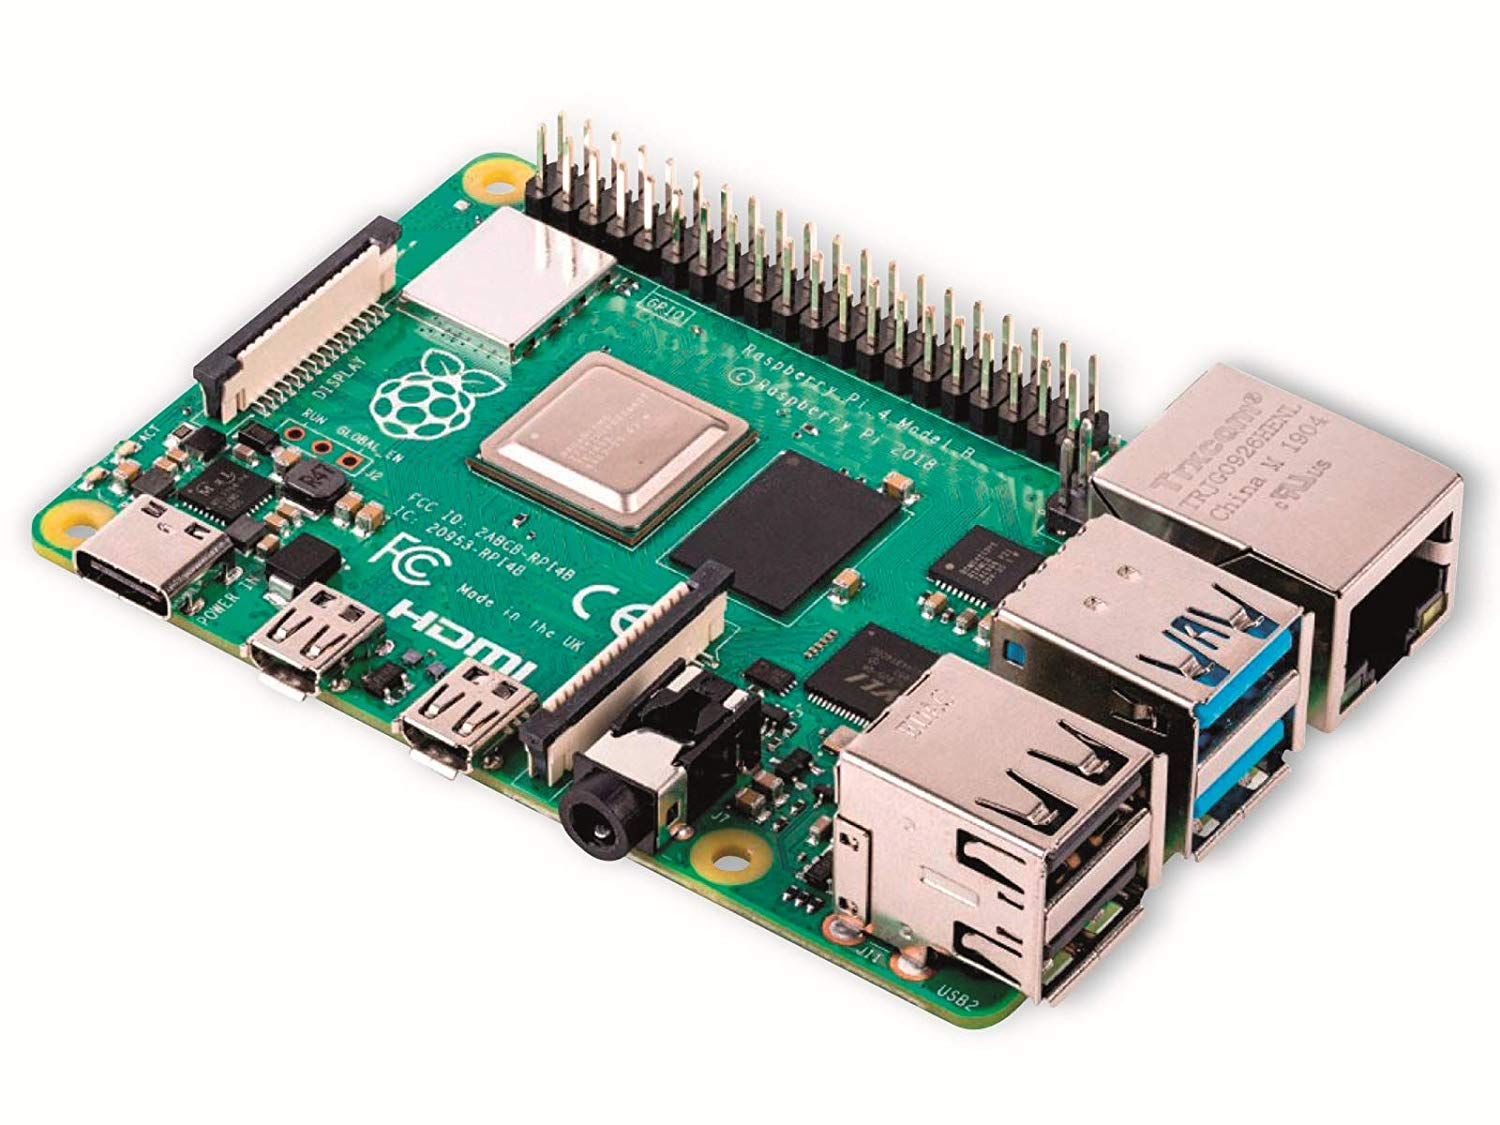
\includegraphics[width=30mm, height=20mm]{raspberry.jpg}
        \end{minipage} 
                & Specifications are enough for our 
                application, support WiFi and its 
                small size and weight is an advantage.\\ 
                \addlinespace

        RPI UPSPack V3 with 4000mAh 
        lithium Battery  
            & \begin{minipage}{.1\textwidth}
                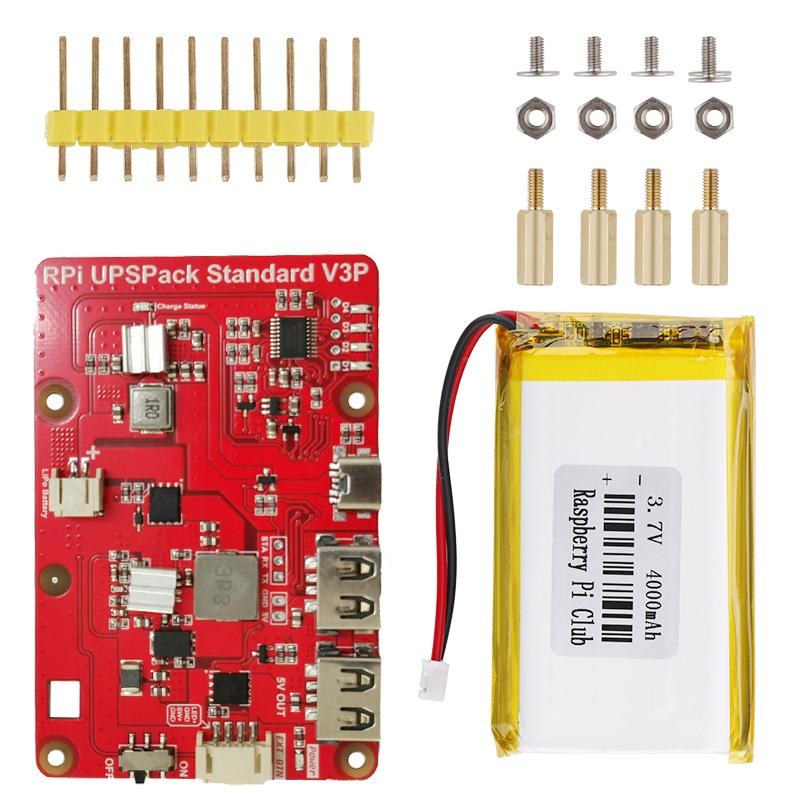
\includegraphics[width=30mm, height=35mm]{RPI.jpg}
        \end{minipage}  
                & Support up to 4 hours which is more 
                than enough , the board got an LED 
                indicator for charging level also the 
                weight and shape is an advantage.  \\ 
                \addlinespace

        Wireless N Nano USB Adapter  
            & \begin{minipage}{.1\textwidth}
                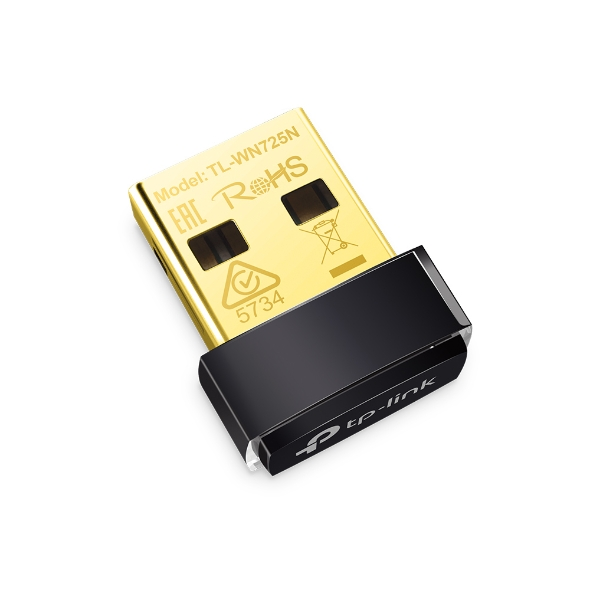
\includegraphics[width=28mm, height=28mm]{dongle.jpg}
        \end{minipage} 
                & Cheap and do its job, good coverage 
                range.  \\ 
                \addlinespace

   Laptop 
            & \begin{minipage}{.1\textwidth}
                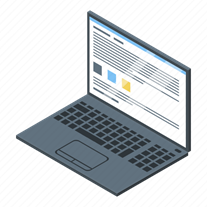
\includegraphics[width=30mm, height=30mm]{laptop.png}
        \end{minipage} 
                & Any laptop with good WiFi interface 
                card will be enough for our case. \\ 
                \addlinespace

        \bottomrule
    \end{tabular}
\end{table}    


\end{document}
